\section{Auswertung}


\subsection{Bestimmung der Kugeldichten}

In der Tabelle \ref{tab:messwerte_kugel} sind die gemessenen
Durchmesser und Massen der Kugeln einzusehen.

\begin{table}
\centering
\begin{tabular} {ccccccc} %Hier noch Radius durch Durchmesser ändern.
	\toprule
  & \multicolumn{3}{c}{Durchmesser in $\si{\meter}\cdot \num{e-3}$}  & \multicolumn{3}{c}{Masse in $\si{\kilogram}\cdot \num{e-3}$} \\
\midrule 
Kugel 1 & $\num{15.13} $&  $\num{15.125} $ & $\num{15.13} $  & $\num{4.45}$ & $\num{4.44} $ & $\num{4.44} $ \\
Kugel 2  & $\num{15.30} $&  $\num{15.30} $ & $\num{15.30} $ & $\num{4.6}$ & $\num{4.6} $ & $\num{4.61} $ \\
\bottomrule
\end{tabular}
\caption{Abmessung der Kugeln}
\label{tab:messwerte_kugel}
\end{table}

Der Radius wird dann mit
\begin{equation*}
r=\frac{d}{2}
\end{equation*}
bestimmt.

Der Mittelwert der Messreihen wird mittels

\begin{equation}
\label{eq:mittel}
\bar{x}=\frac{1}{n}\sum_{i=1}x_i
\end{equation}

bestimmt. Dabei wird der zugehörige Fehler
durch
\begin{equation}
\label{eq:stand_ab}
\Delta \overline{x}=\sqrt{\frac{1}{n(n-1)}\sum_{i=1}^{n}(x_i-\bar{x})^2}.
\end{equation}

berechnet.
Außerdem wird die Gaußsche Fehlerfortpflanung

\begin{equation}
\label{eq:gauss}
\Delta f=\sqrt{\sum_{i=0}^n\left(\frac{\partial f}{\partial x_n} \Delta x_n\right)^2}
\end{equation}

benutzt.
Für die Messungen aus \ref{tab:messwerte_kugel} ergeben sich die
folgenden Werte:

\begin{align} %Hier noch Genauigkeit erhöhen und Durchmesser angeben
\label{eq:abmessungen_kugel}
\begin{aligned}
\overline{m}_{1}&=  \num{0.00444}\si{\kilogram} \\
\overline{m}_{2}&= \num{0.00460} \si{\kilogram} \\
\hfill \\
\overline{d}_{1}&= \num{0.0151}\si{\meter} \\
\overline{d}_{2}&= \num{0.0153} \si{\meter} \\
\hfill\\
\overline{r}_{1}&= \num{0.0076}\si{\meter} \\
\overline{r}_{2}&= \num{0.0077} \si{\meter} \\
\end{aligned}
\end{align}

Der Fehler der Größen in \eqref{eq:abmessungen_kugel} ist in Größenordnung $\pm \num{e-6}\, \si{\kilogram}\, \,\text{bzw.}\, \, \si{\meter}$
und wurde deshalb nicht mit aufgeführt.

Mithilfe der Formel%ausdruck

\begin{equation*}
\rho=\frac{m}{V_{k}} \qquad \text{mit} \, V_{k}=\frac{4}{3}\pi \left(\frac{d}{2}\right)^3
\end{equation*}

können die Dichten der Kugeln ermittelt werden.
Es ergibt sich:

\begin{align*}
\rho_{1}&=\left(\num{2451.0}\pm\num{1.64}\right) \si{\kilogram\per\cubic\meter}\\
\rho_{2}&=\left(\num{2454.7}\pm\num{1.44}\right) \si{\kilogram\per\cubic\meter}
\end{align*}
Die Fehler wurden mit \eqref{eq:gauss} bestimmt.
\subsection{Bestimmung der Viskosität von Wasser bei Zimmertemperatur} \label{sec:visko}
Um die Viskosität zu bestimmen, wird die Dichte von Wasser und die Fallzeit der kleinen Kugel benötigt.
Die gemessenen Werte sind in Tabelle \ref{tab:messwerte_fallzeit_kugel_klein} aufgelistet. %auf
\begin{table} %Hier noch die Genauigkeit erhöhen
\centering
\begin{tabular} {c}
	\toprule
  Fallzeit $t_1$ in $\si{\second}$ \\
  \midrule
  $\num{12.7}$ \\
  $\num{12.76}$ \\
  $\num{12.89}$ \\
  $\num{12.76}$ \\
  $\num{12.83}$ \\
  $\num{12.80}$ \\
  $\num{12.70}$ \\
  $\num{12.67}$ \\
  $\num{12.73}$ \\
  $\num{12.81}$ \\
\bottomrule
\end{tabular}
\caption{Fallzeiten der kleinen Kugel im Viskosimeter bei $\SI{20}{\degreeCelsius}$}
\label{tab:messwerte_fallzeit_kugel_klein}
\end{table}
\\
\\
\hfill
Als gemittelter Wert ergibt sich

\begin{equation}
\label{eq:gemittelte_fallzeit_klein}
\overline{t}_{1}=\left(\num{12.77}\pm\num{0.02}\right) \si{\second}.
\end{equation}

Mittels der Gleichung \eqref{eq: eta} kann die Viskosität
von Wasser bei $\SI{20}{\degreeCelsius}$ bestimmt werden.
Als Wert errechnet sich:

\begin{equation}
\label{eq:viskosi_wasser}
\eta_{20}= \num{0.0014} \si{\pascal\second}
\end{equation}

Der Fehler für die Viskosität liegt in der Größenordnung $\pm\SI{e-6}{\pascal\second}$. %genau bei {e-6} ?

Für die Dichte von Wasser bei $\SI{20}{\degreeCelsius}$ wurde der Literaturwert $\rho_{20}=\SI{998.21}{\kilogram\per\cubic\meter}$
genutzt\cite{lit_dichte}.

\subsection{Bestimmungen der Apperaturkonstante für die große Kugel}
Für die Bestimmung der Apperaturkonstante der großen Kugel nutzt man Gleichung \eqref{eq: eta}.

\begin{equation*}
\Leftrightarrow \quad K_{g}=\frac{K_{kl}\left(\rho_1-\rho_{20}\right)\overline{t}_1}{\left(\rho_2-\rho_{20}\right)\overline{t}_2}
\end{equation*}

Hierbei sei $\overline{t}_2$ die Fallzeit der zweiten Kugel.
Der Fehler der Größe $K_{g}$ wird mittels Gaußscher Fehlerfortpflanzung berechnet.
Die aufgenommenen Messwerte sind in Tabelle \ref{tab:messwerte_fallzeit_kugel_gross} dargestellt.

\begin{table}
\centering
\begin{tabular} {c}
  \toprule
  Fallzeit $t_2$ in $\si{\second}$ \\
  \midrule
  $\num{97.30}$ \\
  $\num{97.60}$ \\
  $\num{97.41}$ \\
  $\num{97.83}$ \\
  $\num{97.16}$ \\
  $\num{97.30}$ \\
  $\num{97.16}$ \\
  $\num{97.28}$ \\
  $\num{97.61}$ \\
  $\num{97.72}$ \\
\bottomrule
\end{tabular}
\caption{Fallzeiten der großen Kugel im Viskosimeter bei $\SI{20}{\degreeCelsius}$}
\label{tab:messwerte_fallzeit_kugel_gross}
\end{table}

Als gemittelte Zeit ergibt sich:
\begin{equation}
\label{eq:gemittelte_fallzeit_gross}
\overline{t}_{2}=\left(\num{97.44}\pm\num{0.075}\right) \si{\second}.
\end{equation}

Mit dem Ergebnis aus \eqref{eq:viskosi_wasser} ergibt sich für die
Apperaturkonstante

\begin{equation}
\label{eq:app_konst_gross}
K_{g}=\left(\num{9.98}\pm\num{0.02}\right)\cdot{\num{e-9}} \si{\pascal\cubic\meter\per\kilogram}.
\end{equation}
Der Fehler wird mittels Gauß berechnet.

\subsection{Bestimmung der Viskosität in Abhängigkeit von der Temperatur}
Mit der gefundenen Konstante $K_{g}$ und den temperaturabhängigen Dichten kann nun die dynamische 
Viskosität berechnet werden. %Satz gefällt mir noch nicht... vielleicht: Mit der gefundenen Konstante K und der temperaturabhängigen Dichte(ref) kann nun die dynamische Viskosität berechnet werden.
Lediglich die Dichte von Wasser ist nun temperaturabhängig.
Aus der Literatur wurde die in Tabelle \ref{tab:dichtewasser} dargestellten Werte
entnommen \cite{lit_dichte}.  %Noch literatur ref

\begin{table}
\centering
\begin{tabular} {cc}
  \toprule
  Temperatur in $\si{\kelvin}$ & Dichte $\rho$ in $\si{\kilogram\per\cubic\meter}$ \\
  \midrule
  $\num{303.16}$ &$\num{995.65}$ \\
  $\num{308.16}$ &$\num{994.00}$\\
  $\num{313.16}$ &$\num{992.20}$\\
  $\num{318.16}$ &$\num{990.20}$\\
  $\num{323.16}$ &$\num{988.00}$\\
  $\num{328.16}$ &$\num{985.70}$\\
  $\num{333.16}$ &$\num{983.20}$\\
  $\num{338.16}$ &$\num{980.60}$\\
  $\num{343.16}$ &$\num{977.8}$\\
\bottomrule
\end{tabular}
\caption{Temperaturabhängige Dichte von Wasser}
\label{tab:dichtewasser}
\end{table}

Bei den späteren Berechnungen wird für die Dichte von Wasser, bei den Temperaturen $\SI{336.16}{\kelvin}$ und $\SI{339.16}{\kelvin}$
der Wert $\SI{983.20}{\kilogram\per\cubic\meter}$ verwendet. %verwendet

Für die Fallzeit der Kugel ergeben sich die in  %würde tempus einheitlich machen
Tabelle \ref{tab:messwerte_fallzeit_kugel_gross_temo} aufgelisteten Werte.

\begin{table}
\centering
\begin{tabular} {cccc}
  \toprule
  Temperatur in $\si{\kelvin}$ & \multicolumn{2}{c}{Fallzeit $t$ in $\si{\second}$} & $\overline{t}$ in $\si{\second}$ \\
  \midrule
  $\num{303.16}$ & $\num{96.92}$  & $\num{97.04}$ & $\num{96.98}\pm\num{0.06}$ \\
  $\num{308.16}$ & $\num{93.58}$  & $\num{93.73}$ & $\num{93.66}\pm\num{0.05}$ \\
  $\num{313.16}$ & $\num{92.63}$ & $\num{92.95}$   & $\num{92.79}\pm\num{0.11}$ \\
  $\num{318.16}$ & $\num{90.36}$ & $\num{90.45}$ &  $\num{90.41}\pm\num{0.03}$ \\
  $\num{323.16}$ & $\num{87.73}$ & $\num{87.55}$ & $\num{87.64}\pm\num{0.06}$ \\
  $\num{328.16}$ & $\num{83.36}$ & $\num{83.44}$ & $\num{83.40}\pm\num{0.03}$ \\
  $\num{333.16}$ & $\num{81.38}$ & $\num{81.35}$ & $\num{81.37}\pm\num{0.01}$ \\
  $\num{336.16}$ & $\num{79.61}$ & $\num{79.61}$ & $\num{79.61}\pm\num{0.00}$ \\
  $\num{339.16}$ & $\num{78.01}$ &  $\num{77.63}$ & $\num{77.82}\pm\num{0.13}$ \\
  $\num{343.16}$ & $\num{73.04}$ & $\num{73.18}$ & $\num{73.11}\pm\num{0.05}$ \\
\bottomrule
\end{tabular}
\caption{Temperaturabhängige Fallzeiten der großen Kugel im Viskosimeter} %ausdruck
\label{tab:messwerte_fallzeit_kugel_gross_temo}
\end{table}

Das Ergebnis der Viskositätsberechnung (nach \eqref{eq: eta}) ist in Tabelle \ref{tab:visko_wasser_temp} zu finden. % zu finden
Die Fehler der Berechnungen ist in der Größenordnung $\pm \SI{e-6}{\pascal\second}$ und 
wird deshalb nicht aufgeführt.

\begin{table}
\centering
\begin{tabular} {ccc}
  \toprule
  Temperatur in $\si{\kelvin}$ & Viskosität $\eta\cdot\num{e-3}$ in $\si{\pascal\second}$ & Literaturwerte $\eta_{lit}\cdot\num{e-3}$ in $\si{\pascal\second}$  \\
  \midrule
  $\num{303.16}$ & $\num{1.41}$ & $\num{0.801}$  \\
  $\num{308.16}$ & $\num{1.37}$ & $\num{0.723}$  \\
  $\num{313.16}$ & $\num{1.35}$& $\num{0.656}$  \\
  $\num{318.16}$ & $\num{1.32}$ & $\num{0.599}$\\
  $\num{323.16}$ & $\num{1.28}$& $\num{0.549}$ \\
  $\num{328.16}$ & $\num{1.22}$& $\num{0.506}$ \\
  $\num{333.16}$ & $\num{1.20}$& $\num{0.468}$ \\
  $\num{336.16}$ & $\num{1.17}$&  --- \\
  $\num{338.16}$ & --- & $\num{0.436}$ \\
  $\num{339.16}$ & $\num{1.14}$&  --- \\
  $\num{343.16}$ & $\num{1.08}$& $\num{0.406}$ \\
\bottomrule
\end{tabular}
\caption{Dynamische Viskosität} %ausdruck
\label{tab:visko_wasser_temp}
\end{table}

Die Ergebnisse werden in Abbildung \ref{fig:t_v_v} und \ref{fig:t_v_l_v} dargestellt.
In den Abbildung \ref{fig:t_v_v} wird die Temperatur gegen die Viskosität aufgetragen.
Zusätzlich werden die Literaturwerte \cite{lit_dichte} mit aufgetragen.
Dagegen wird in Abbildung \ref{fig:t_v_l_v} $\log(\eta)$ gegen $\frac{1}{T}$ aufgetragen.
Darüberhinaus sind auch die Literaturwerte \cite{lit_dichte} mit abgebildet.
Zur Berechnung der Ausgleichsgeraden in \ref{fig:t_v_l_v} , wurde aus der Regressionsrechnung:

\begin{equation*}
m=\frac{\overline{xy}-\bar{x}\bar{y}}{\bar{x^2}-\bar{x}^2}
\end{equation*}
zur Bestimmung der Steigung, mit dem dazugehörigen Fehler

\begin{equation*}
\sigma_m=\sqrt{\frac{\sigma^2}{N(\bar{x^2}-\bar{x}^2)}}
\end{equation*}

benutzt.
Für den $y$-Achsenabschnitt gilt der Zusammenhang

\begin{equation*}
b=\frac{\bar{x^2}\bar{y}-\bar{x}\bar{xy}}{\bar{x^2}-\bar{x}^2}
\end{equation*}

mit der dazugehörigen Abweichung

\begin{equation*}
\sigma_b=\sqrt{\frac{\sigma^2}{N\left(\bar{x^2}-\bar{x}^2\right)}}.
\end{equation*}
%Ergebnisse, verglichen werden sie doch erst in der diskussion

Für die Abbildung \ref{fig:t_v_v} wurde mittels der Python Bibliothek \emph{Scipy} eine
Regression an eine Funktion der Form $T_i = Ae^{\frac{B}{T}}$ (siehe \eqref{eq: andrad}) bestimmt. %hinter formel ref

Als Parameter ergeben sich:
\begin{equation}
 \label{eq:reg_wert} %Hier nochmal kontrollieren
A=\left(\num{1.74}\pm\num{24.8}\right)\cdot\num{e-4}\,\si{\pascal\second} \quad B=\left(\num{6.396} \pm\num{0.458}\right)\cdot\num{e+2}\,\si{\kelvin} %Einheiten ? haben die ne dimension?
\end{equation}

Für den in Abbildung \ref{fig:t_v_l_v} dargestellten Fit der Messwerte ergeben sich
folgende Parameter:

\begin{equation}
\label{eq:lreg}
A=\left(\num{-8.71}\pm\num{0.15}\right) \quad B=\left(\num{6.6} \pm\num{0.5}\right)\cdot\num{e+2}\,\si{\kelvin} 
\end{equation}

Eine qualitativer Vergleich erfolgt anschließend in der Diskussion. %

\FloatBarrier
\begin{figure}
\centering
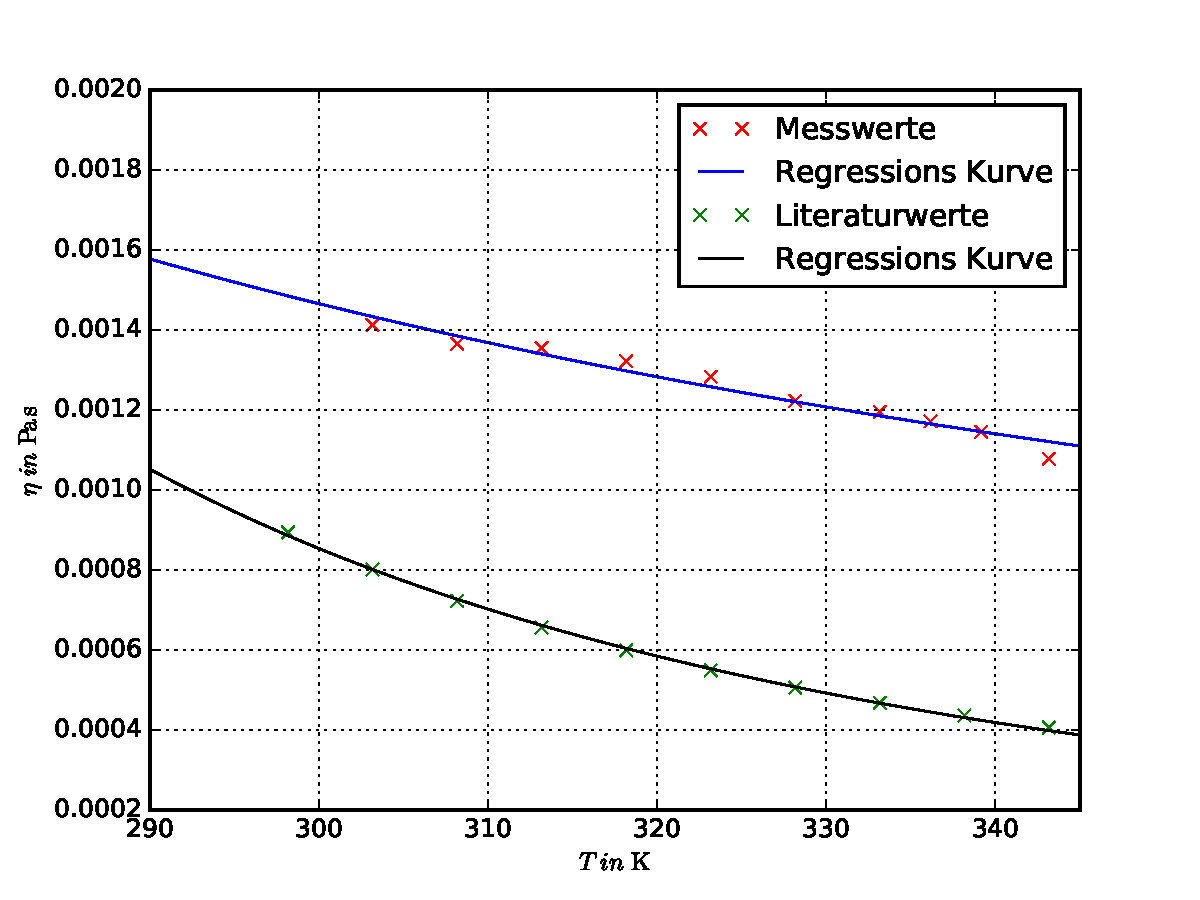
\includegraphics[width=0.7\textwidth]{pics/viskositaet_temp_mit_lit.pdf}
\caption{Auftragung der temperaturabhängigen Viskosität} %umgangssprachlich
\label{fig:t_v_v}
\end{figure}

\begin{figure}
\centering
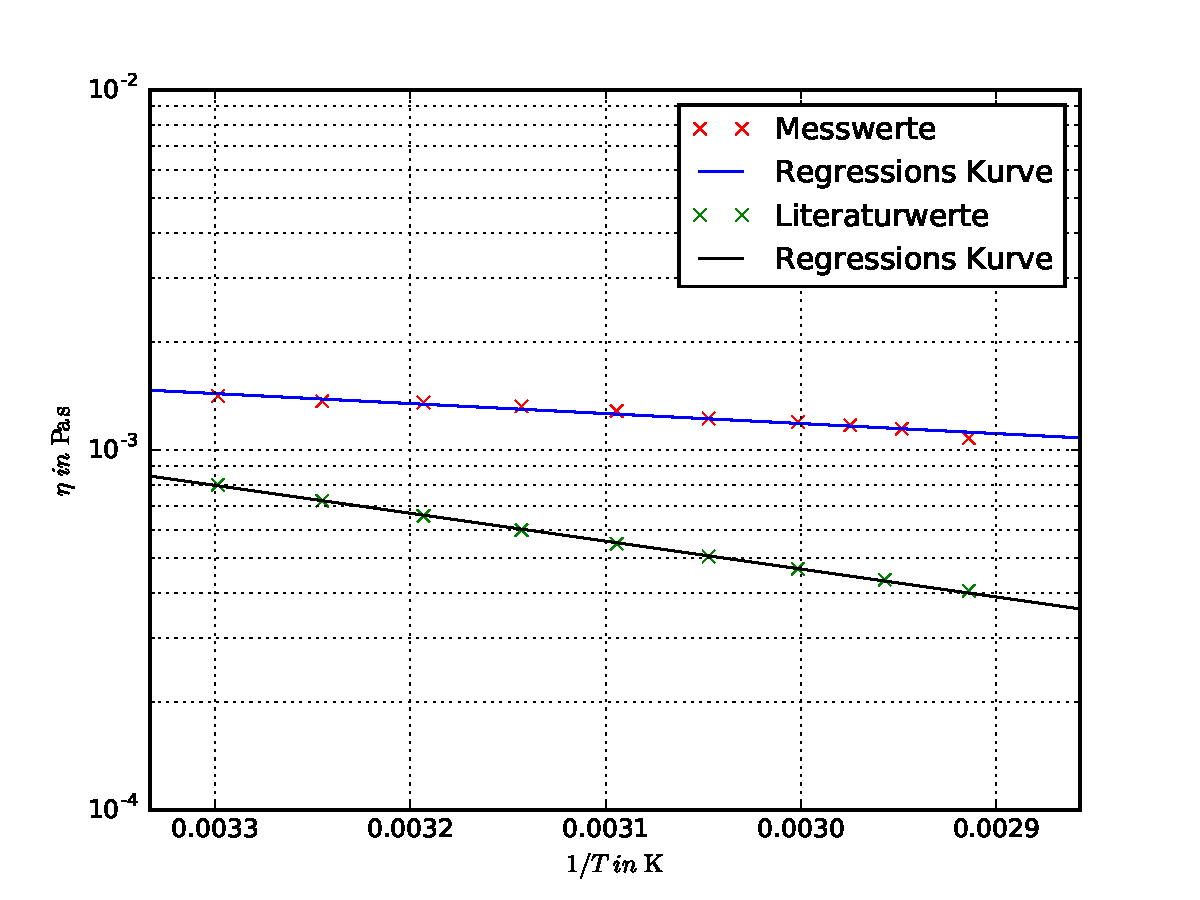
\includegraphics[width=0.7\textwidth]{pics/viskositaet_temp__log_mit_lit.pdf}
\caption{ Auftragung von 1/Temperatur gegen Viskosität (Halblogarithmische Skala)} %Überprüfen
\label{fig:t_v_l_v}
\end{figure}
\FloatBarrier



\subsection{Bestimmung der Reynolds-Zahl}

Die \emph{Reynolds-Zahl} wird durch die Gleichung \eqref{eq: reynolds} bestimmt.
Dabei wird $v_0$ ersetzt durch $v_0=\frac{l}{t}$.
Zusätzlich sei $d$ der Rohrdurchmesser  %verb
Der Rohrdurchmesser wird durch den Durchmesser der großen Kugel genährt.
Die Fehler der \emph{Reynolds-Zahl} werden nach Gauß berechnet. %genähert

%Die temperaturabhängigen Fallgeschwindigkeiten der Kugel ist in Tabelle 
%\ref{tab:fall_kugel} einzusehen.
%Da Fehler der Geschwindigkeitsberechnung in der Größenordnung $\num{e-6}$ ist,
%wird er nicht mit aufgelistet.

%\begin{table}
%\centering
%\begin{tab%ular} {cc}
%  \toprule
%  Temperatur in $\si{\kelvin}$ & Fallgeschwindigkeit $v$ in $\si{\meter\per\second}$ \%\
%  \midrule
%  $\num{303.16}$ & $\num{0.00103}$ \\
%  $\num{308.16}$ & $\num{0.00107}$ \\
%  $\num{313.16}$ & $\num{0.00108}$ \\
%  $\num{318.16}$ & $\num{0.00110}$ \\
%  $\num{323.16}$ & $\num{0.00114}$ \\
%  $\num{328.16}$ & $\num{0.0012}$ \\
%  $\num{333.16}$ & $\num{0.00123}$ \\
%  $\num{336.16}$ & $\num{0.001126}$ \\
%  $\num{339.16}$ & $\num{0.00129}$ \\
%  $\num{343.16}$ & $\num{0.00137}$ \\
%\bottomrule
%\end{tabular}
%\caption{Fallgeschwindigkeit der großen Kugel bei unterschiedlichen Temperaturen}
%\label{tab:fall_kugel}
%\end{table}

Die Werte für die \emph{Reynolds-Zahl} sind in Tabelle \ref{tab:rey_visko} %'sich damit ergebenen Werte' weglassen
zu finden.

\begin{table}
\centering
\begin{tabular} {cc}
  \toprule
  Temperatur in $\si{\kelvin}$ & \emph{Reynolds-Zahl} $\map{Re}$ \\
  \midrule
  $\num{303.16}$ & $\num{11.1}\pm \num{0.03}$ \\
  $\num{308.16}$ & $\num{11.9}\pm \num{0.03}$ \\
  $\num{313.16}$ & $\num{12.1}\pm \num{0.04}$ \\
  $\num{318.16}$ & $\num{12.7}\pm \num{0.03}$ \\
  $\num{323.16}$ & $\num{13.4}\pm \num{0.03}$ \\
  $\num{328.16}$ & $\num{14.8}\pm \num{0.03}$ \\
  $\num{333.16}$ & $\num{15.5}\pm \num{0.03}$ \\
  $\num{336.16}$ & $\num{16.1}\pm \num{0.03}$ \\
  $\num{339.16}$ & $\num{16.8}\pm \num{0.07}$ \\
  $\num{343.16}$ & $\num{19}\pm \num{0.05}$ \\
\bottomrule
\end{tabular}
\caption{\emph{Reynolds-Zahl} des Viskosimeters bei unterschiedlichen Temperaturen} %viskosimeters
\label{tab:rey_visko}
\end{table}


Bei dem Fall der kleinen Kugel egibt sich eine \emph{Reynolds-Zahl} von:
\begin{equation*}%Hier noch Wert einfügen
\map{Re}_{klein}=\left(\num{84.45}\pm\num{0.29}\right)
\end{equation*}
Die Werte liegen alle unterhalb der in der Theorie angesprochenen kritischen \emph{Reynolds-Zahl}. %auf theorie verweisen
Deshalb handelt es sich um eine laminare Strömung.


%ausdruck
 %Literatur
